%% Change "letterpaper" in the following line to "a4paper" if you must.

\documentclass[10pt,a4paper]{article}
\usepackage{cogsci}
\usepackage{pslatex}
\usepackage{apacite}


%\usepackage{geometry}
\usepackage{natbib}
\bibpunct[:]{(}{)}{,}{a}{}{;}

\usepackage{amsmath}
\usepackage{amsfonts}
\usepackage{amsthm}
\usepackage{amssymb}
\usepackage{mathrsfs}
\usepackage{nicefrac}
%\usepackage{stmaryrd}
%\usepackage{multicol}
\usepackage{graphicx}
\usepackage{caption}
\usepackage{subcaption}
\usepackage{color}
\usepackage{booktabs}

\usepackage{blkarray}
\usepackage{xspace}


\definecolor{Red}{RGB}{178,34,34}
\newcommand{\mf}[1]{\textcolor{Red}{[MF: #1]}} 
\newcommand{\tb}[1]{\textcolor[rgb]{.8,.33,.0}{[TB: #1]}}% prints in orange
\newcommand{\citeposs}[2][]{\citeauthor{#2}'s (\citeyear[#1]{#2})}
\newcommand{\tuple}[1]{\ensuremath{\left\langle #1 \right\rangle}} 


%%% MF's commands
\newcommand{\set}[1]{\left\{#1\right\}}
\newcommand{\card}[1]{\left \lvert \, #1 \, \right\rvert}
\newcommand{\abs}[1]{\lvert #1 \rvert}
\newcommand{\States}{\ensuremath{S}\xspace}		% Set of States
\newcommand{\state}{\ensuremath{s}\xspace}		% single states
\newcommand{\mystate}[1]{\ensuremath{\state_{\text{#1}}}\xspace} %meaningful states
\newcommand{\Messgs}{\ensuremath{M}\xspace}		% Set of Messages
\newcommand{\messg}{\ensuremath{m}\xspace}		% single messages
\newcommand{\mymessg}[1]{\ensuremath{\messg_{\text{#1}}}\xspace} %meaningful messages
\newcommand{\ssome}{\mystate{\ensuremath{\exists\neg\forall}}}
\newcommand{\sall}{\mystate{\ensuremath{\forall}}}
\newcommand{\msome}{\mymessg{some}}
\newcommand{\mall}{\mymessg{all}}
\newcommand{\asome}{\myact{\ensuremath{\exists\neg\forall}}}
\newcommand{\aall}{\myact{\ensuremath{\forall}}}
\definecolor{mygray}{cmyk}{0.35,0.35,0.35,0.35}
\newcommand{\mygray}[1]{{\textcolor{mygray}{#1}}}


%\citeA{bibkeyword} cites only year

\title{Effects of transmission perturbation in the cultural evolution of language}
 
\author{{\large \bf Name Surname (mail@mail.com)} \\
  Department, street \& number \\
  city, ZIP country
  \AND {\large \bf Name Surname (mail@mail.com)} \\
  Department, street \& number \\
  city, ZIP country}


\begin{document}
\maketitle

\begin{abstract}
  Two main factors seem to play a major role in the cultural evolution of language. On the on
  hand, there is functional pressure towards efficient transfer of relevant information. On the
  other hand, languages have to be learned repeatedly and will therefore show traces of
  systematic stochastic perturbations operating during the transmission of linguistic
  knowledge. While a lot of attention has been paid to the effects of cognitive learning biases
  on the transmission of language, there is reason to expect that the class of possibly
  relevant transmission biases is much larger. This paper therefore explores some potential
  effects of transmission noise due to errors in the observation of states of the world. We
  look at three case studies on (i) vagueness, (ii) meaning deflation, and (iii) underspecified
  lexical meaning. These case studies suggest that transmission perturbations other than
  learning biases might explain attested patterns in the cultural evolution of language and
  that transmission perturbations due to perceptual noise may even produce effects very similar
  to learning biases.

\textbf{Keywords:} 
noise; cognitive biases; iterated learning; cultural evolution  
\end{abstract}


\section{Introduction}

Language is shaped by its use and transmission across generations. Linguistic properties
therefore need not necessarily arise and stabilize solely due to functional pressure, such as
the selection of more communicatively efficient behavior, but may also be influenced
and selected for by a pressure for learnability. In the extreme, an unlearnable language
will not make it to the next generation. The effects that (iterated) learning has on language
are often seen as stemming from a combination of general learning mechanisms and inductive
cognitive biases
(e.g. \citealt{griffiths+kalish:2007,kirby+etal:2014,tamariz+kirby:2016}). Proposals of biases
that shape language acquisition abound. Some prominent examples are mutual exclusivity
\citep{merriman+bowman:1989,clark:2009}, simplicity \citep{kirby+etal:2015}, regularization
\citep{hudson+etal:2005}, and generalization
\citep{smith:2011,oconnor:2015}.
%\footnote{Depending on their formulation and the domain(s) they
%  are proposed to apply to, biases may also interact. For instance, a domain-independent bias
%  for simplicity may entail regularization but stand in conflict with mutual exclusivity.}
But
there is good reason to expect that forces other than learning biases may systematically
perturb the transmission of linguistic knowledge and therefore additionally contribute to the shaping
of language by cultural evolution.  In the following we focus on one particular source of perturbation:
agents' imperfect perception of the world. The overall goal of this paper is to give a formalism in which to study the effects of such
perturbations and apply it to three case studies on (i) vagueness, (ii) meaning deflation, and
(iii) underspecified lexical meaning.

\section{Iterated Bayesian learning}

We model the transmission of linguistic knowledge as a process of iterated learning (for recent
overviews see \citealt{kirby+etal:2014, tamariz+kirby:2016}). More specifically, we focus on
iterated Bayesian learning, in which a language learner must infer unobservables, such as the
lexical meaning of a word, from the observable behavior of a single teacher, who is a
proficient language user \citep[e.g.][]{griffiths+kalish:2007,kirby+etal:2007}. The learner
observes instances $\tuple{s,m}$ of overt language use in context, where $s$ is a world state
and $m$ is the message that the teacher used in state $s$. The learner's task is to infer which
latent type $t$, e.g., which set of lexical meanings, may have produced a sequence of such
observations. To do so, the learner considers the posterior probability of type $t$ given a
data sequence $d$ of $\tuple{s, m}$ pairs:
\begin{align*}
  P(t \mid d) \propto P(t) \ P(d \mid t)\,,
\end{align*}
where $P(t)$ is the learner's prior for type $t$ and
$P(d \mid t) = \prod_{\tuple{s,m} \in d} P(m \mid s, t)$ is the likelihood of type $t$
producing the observed data $d$, with $P(m \mid s, t)$ the probability that a type $t$ produces
message $m$ when in world state $s$. Models of iterated Bayesian learning usually assume that
the learner adopts a type with a probability proportional to $P(t \mid d)^l$, where $l \ge 1$
is a parameter that regulates whether learners use probability matching ($l = 1$) or show
tendency towards choosing a maximum of the posterior distribution ($l > 1$). 

The set of possible data a learner may be exposed to is the set $D_k$ of all sequences $d$  of $\tuple{s,m}$ pairs with
length $k$. The lower $k$, the less information the learner has at her disposition to
recover the true type of the teacher. Putting these components together in a transmission matrix, $Q_{ji}$ is the probability that a learner acquires type $i$ when learning from type $j$:
\begin{align*}
  Q_{ji} &\propto \sum_{d \in D_k} P(d \mid t_j) F(t_i \mid d)\,, \text{where} \\
  F(t_i \mid d) &\propto [P(t_i) P(d \mid t_i)]^l\,.
\end{align*}


The prior $P(t)$ can be understood as a encoding learning biases. For example, learners may
have a preference for simpler languages over ones with a more complex grammar, larger or more
marked inventories, or cognitively taxing components
(c.f. \citealt{feldman:2000,chater+vitanyi:2003, kirby+etal:2015}). Crucially, even weak biases
can magnify and have striking effects on an evolving linguistic system. Experimental and
mathematical investigations in iterated learning have therefore argued that the linguistic
structure evinced by the outcome of this process reflects learners' inductive biases
\citep{kirby+etal:2007,kirby+etal:2014}. 

%The role of such biases can be viewed as that of
%introducing systematic perturbations in the transmission of linguistic knowledge, guiding
%learners to the convergence on particular evolutionary outcomes.

\section{Iterated Bayesian learning with state-noise}

Other stochastic factors beyond learning biases in $P(t)$ can influence the adoption of a
linguistic type $t$ based on the observation of $\tuple{s,m}$ pairs. One further potential source
of ``transmission noise'' are regular stochastic errors in the perception of world states (see
Figure~\ref{fig:cartoon}).
%
\begin{figure}[t]
  \centering
  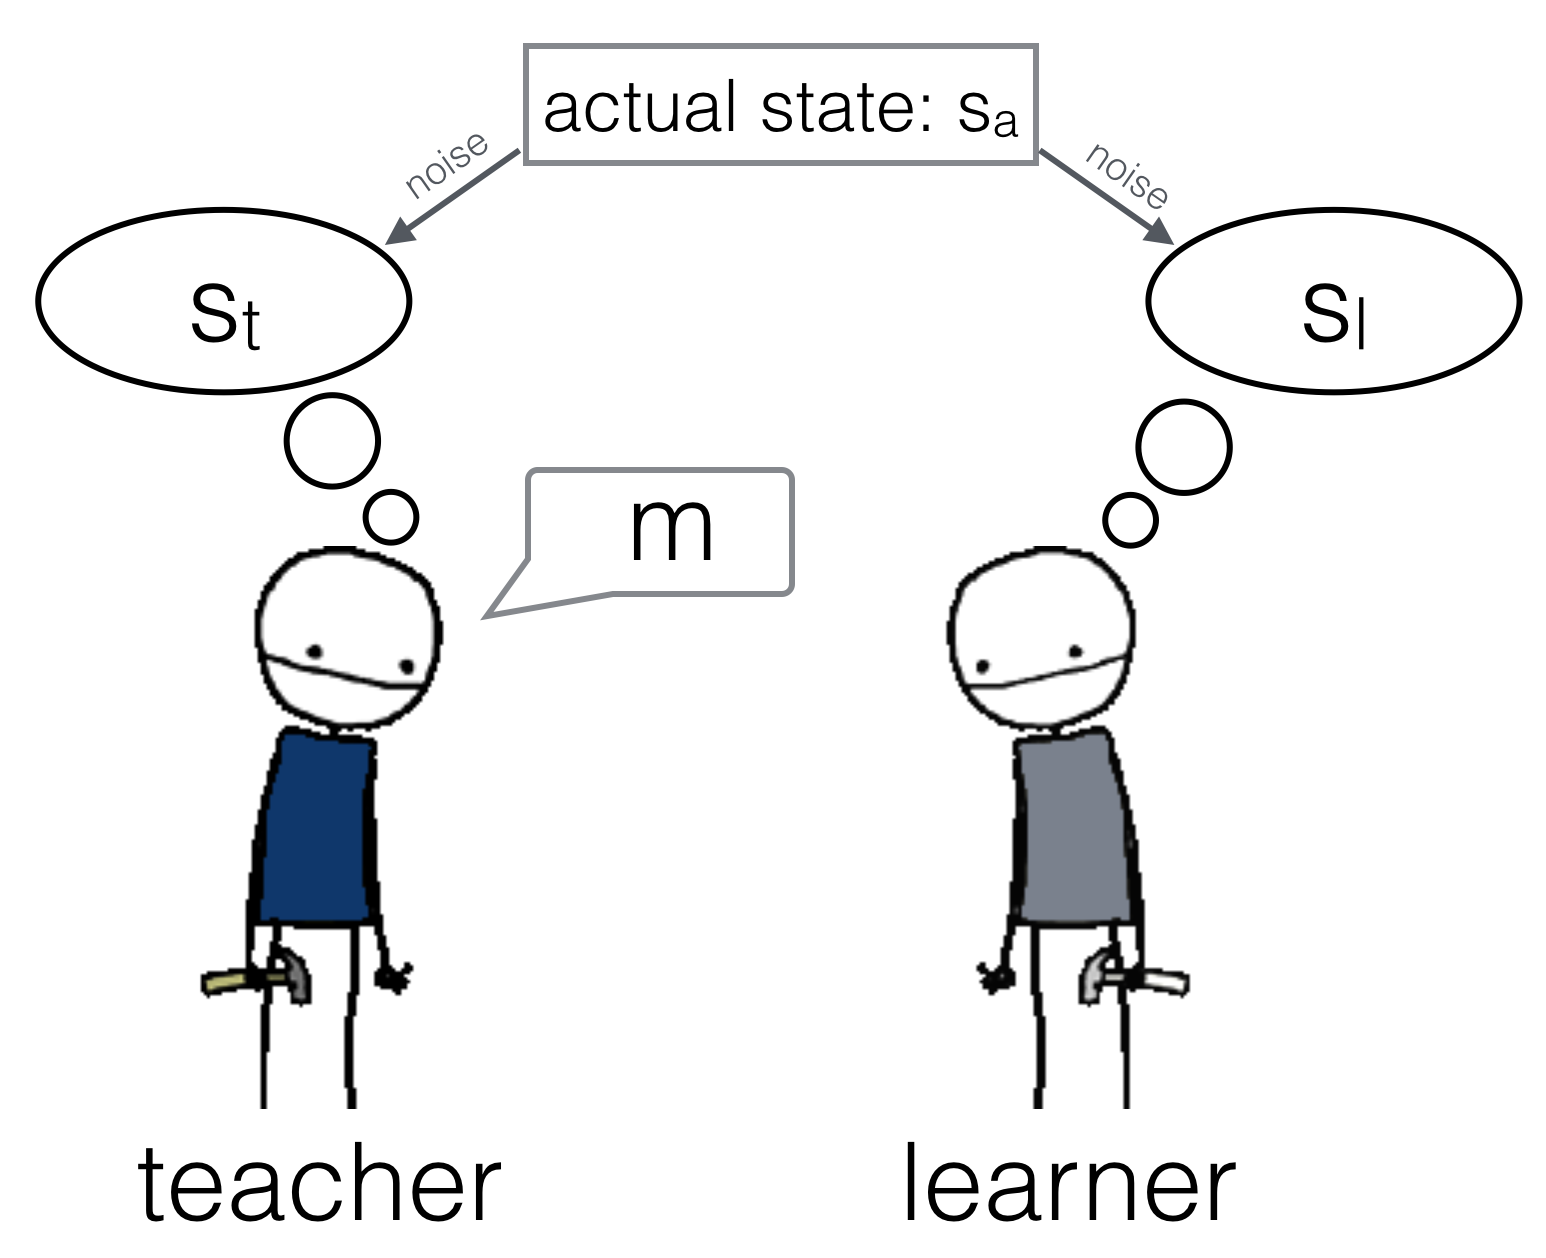
\includegraphics[width = 0.75\linewidth]{pics/cartoon_picture.png}
  \caption{State-noise during observation of language use.}
  \label{fig:cartoon}
\end{figure}
% 
Imperfect perception of world states
may lead teachers to produce utterances that deviate from their production behavior had they
witnessed the state correctly. Similarly, learners may mistake utterances as applying to 
different states than the ones witnessed by the teacher who produced them. For instance, when learning the meaning of a vague adjective
such as {\em tall} from an utterance like ``John is tall,'' agents may have diverging
representations of how tall John actually is, even if he is in a shared perceptual
environment. The main idea to be explored here is that regularities in state-misperceptions may
have striking and possibly explanatory effects on language evolution. 

Let $S$ be a set of world states. We denote the probability that the teacher (learner) observes state $s_t$ ($s_l$) when the actual state is $s_a$ as $P_N(s_t \mid s_a)$ ($P_N(s_l \mid s_a)$). The probability that $s_a$ is the actual state when the learner observes $s_l$ is therefore:
\begin{align*}
  P_N(s_a \mid s_l) \propto P(s_a) \ P_N(s_l \mid s_a)\,.
\end{align*}
Accordingly, the probability that the teacher observes $s_t$ when the learner observes $s_l$ is:
\begin{align*}
  P_N(s_t \mid s_l) = \sum_{s_a} P(s_a \mid s_l) \ P_N(s_t \mid s_a)\,.
\end{align*}
The probability that a teacher of type $t$ produces data that is perceived by the learner as a
sequence $d_l$ of $\tuple{s_l, m}$ pairs is:
\begin{align*}
  P_N(d_l \mid t) = \prod_{\tuple{s_l,m} \in d_l} \sum_{s_t} P_N(s_t \mid s_l) \ P(m \mid s_t; t)\,.
\end{align*}
It is natural to assume that learners, even if they (in tendency) perform rational Bayesian
inference on the likely teacher type $t$ based on observation $\tuple{s_l,m}$, do not also
reason about state-noise perturbations. In this case the posterior probability of $t$ given
the learner's perceived data sequence $d_l$ is as before:
\begin{align*}
  P(t \mid d_l) \propto P(t) \ P(d_l \mid t)\,.
\end{align*}
Still, state-noise affects the probability $Q_{ji}$ that the learner adopts type $i$ given 
a teacher of type $j$, because it influences the probability of observing a sequence $d_l$:
\begin{flalign*}
  Q_{ji} \propto \sum_{d \in D_k} P_N(d_l \mid t_j) F(t_i \mid d)\,,
\end{flalign*}
where $F(t_i \mid d)$ is as before.

Noise free iterated Bayesian learning is obtained as a special case when the perceived state is
always the actual state.

% Finally, we need to specify what the transmission matrix $Q$ operates over. This could be a distribution over types that an agent in the learning chain entertains at a given time, but also as a population of types following standard practice in evolutionary game theory (for discussion on the relationship of single chain learning and population dynamics see e.g. \citealt[\S 7]{griffiths+kalish:2007}). Here, we adopt the latter view, and consequently take this component to be a population vector $x$, where $x_i$ is the proportion of type $t_i$ in $x$. The full dynamics are captured by the discrete mutator dynamics $\hat{x}_j = \sum_i Q_{ij} x_j$ (for an overview see \citealt{hofbauer+sigmund:2003}).

In sum, it may be the case that learner and/or teacher do not perceive the actual state as what
it is. They are not aware of this, and produce/learn as if what they observed was the actual
state. The learner does not reason about noise when she tries to infer the
speaker's type. She takes what she observes a state to be as the actual state that the teacher
has seen as well and infers which type would have most likely generated the message to this
state. This can lead to biases of inferring the ``wrong'' teacher type if the noise makes some
types err in a way that resembles the noiseless behavior of other types. That is, such
environmental factors can, in principle, induce transmission perturbations that look as if there was a
cognitive bias in favor of a particular type, simply because that type better explains the
noise.


\section{Case studies}

In what follows we present three case studies that show how iterated learning under noisy
perception of states can lead to the emergence of linguistic phenomena found in natural
language. Case studies are ordered from more to less obvious examples in which state-noise may
help explain phenomena of interest: (i) vagueness, (ii) meaning deflation, and (iii)
underspecification in the lexicon.
% The first study on vagueness shows that, if concerns the emergence of vagueness in a community of language users
% that initially makes sharp linguistic distinctions between states. The second study considers a
% similar setup in which agents start out by using an expression only for a small subset of
% states. Over time, the strict boundary set by the initial language is shown to relax, leading
% to an iterated expansion of the expression's range over the state space. That is, meaning
% deflates as a consequence of transmission perturbations caused by noise. Finally, we analyze a
% subset of \citeposs{brochhagen+etal:2016:CogSci} case study on the lexicalization of a lack of
% upper-bounds in the meaning of weak scalar expressions. As in the preceding cases, we show how
% certain noise patterns can give rise to outcomes predicted by theoretical and empirical
% investigations.
No case study is meant to suggest that state-noise is the definite answer to the question of
how this property arose. Instead, we restrict our attention to minimal settings that
deliberately abstract away from aspects not required for our present aim, which is to elucidate
the role that transmission perturbations beyond inductive biases may play in shaping the
cultural evolution of language.

%Note also that constructing the set of learning data $D$ is computationally intractable for
%large $k$. We therefore approximate $D$ by sampling data from the production behavior of
%types. The values chosen correspond to experimentally determined amounts that minimize the
%effects that insufficient sampling may otherwise introduce. \mf{I would probably skip
%  this. Technical details are backgrounded here anyway, and have to be.}

\subsection{Vagueness}

Many if not most expressions in natural language are vague. Vagueness should be distinguished
from imprecision and genuine ambiguity. The hallmark of vagueness is susceptibility to a
Sorites paradox \citep[e.g.][]{Williamson1994:Vagueness}: if a car for one million US\$ is
expensive, and if additionally a car that costs a single dollar less than an expensive car is still expensive,
then it is also true that a car for one US\$ is expensive. Vague expressions fall prey to this fallacious reasoning pattern.

Vagueness also poses serious challenges to models of language evolution since functional
pressure towards maximal information transfer should, under fairly general conditions, work
against vagueness \citep{Lipman2009:Why-is-Language}. Many have therefore argued
that vagueness is intrinsically useful for communication
\citep[e.g.][]{Deemter2009:Utility-and-Lan,Jaegherde-JaegherRooijvan-Rooij2010:Strategic-Vague,BlumeBoard2013:Intentional-Vag}. Others
hold that vagueness arises naturally due to limits in perception, memory, or information
processing
\citep[e.g.][]{FrankeJager2010:Vagueness-Signa,LassiterGoodman2015:Adjectival-vagu,OConnor2013:The-Evolution-o}. We
follow the latter line of exploration here, arguing that vagueness arises naturally under
imperfect observability of states (see \cite{franke+correia:toappear} for an imitation-based
dynamic based on the same idea).

\mf{rewrite up to here}

\paragraph{Setup.}  We analyze the effects noisy perception has on the transmission of a simple language with $100$
states, $s \in [0,99]$, and two messages, $m \in \{m_1,m_2\}$. The probability of perceiving the
actual state $s_a$ as $s_p$ is given by a truncated normal distribution with the actual state as its mean, 
a standard deviation $\sigma$ and a truncation range $[0,99]$. That is, $P(s_p | s_a) \sim \text{Normal}(s_{a},\sigma,s_{0},s_{99})$
with $\sigma$ controlling the degree to which states are confused, and as boundaries $s_{0}$ and $s_{99}$. Linguistic behavior is assumed to be uniform across speakers and to depend solely on a type $t_i$'s index, $i \in [0,99]$. This index indicates which message a type uses in a (perceived) state: If $s_j$ is the $j$-th state, then $P(m_1|s_j,t_i) = 1$ iff $j \geq i$. Otherwise, $P(m_2|s_j,t_i) = 1$. In words, if the state is perceived to be as large or larger than a type's index, then message $m_1$, e.g., {\em tall}, is used. Otherwise $m_2$, e.g., {\em small}, is used.

\paragraph{Results.} The effects of a single generational turnover under noisy transmission is depicted in Figure \ref{fig:vagb}. As shown in Figure \ref{fig:vaga}, this population initially consisted exclusively of type $t_{50}$. \tb{Do you think it might be confusing to start speaking about populations here? We now don't have a paragraph mentioning what evolves explicitly} As learners try to acquire this type, even small $\sigma$ will lead to the emergence of vagueness. The same outcome is obtained for other values of $\sigma$ with higher values leading to more borderline cases that do not clearly fall under either only $m_1$ or $m_2$. Here, iterated noisy transmission leads to mixed populations and, consequently, to convex areas of the state space not clearly associated with a particular form. The size of the space devoted to such borderline cases increases over generations with its growth being inversely related to $l$ and $k$. As is to be expected, if $k$ is too small to discern even strikingly different types, then iterated learning under noisy perception leads to heterogeneous populations with (almost) no state being exclusively associated with $m_1$ or $m_2$.

\begin{figure}[ht]
  \centering
  \begin{subfigure}[b]{0.45\textwidth}
    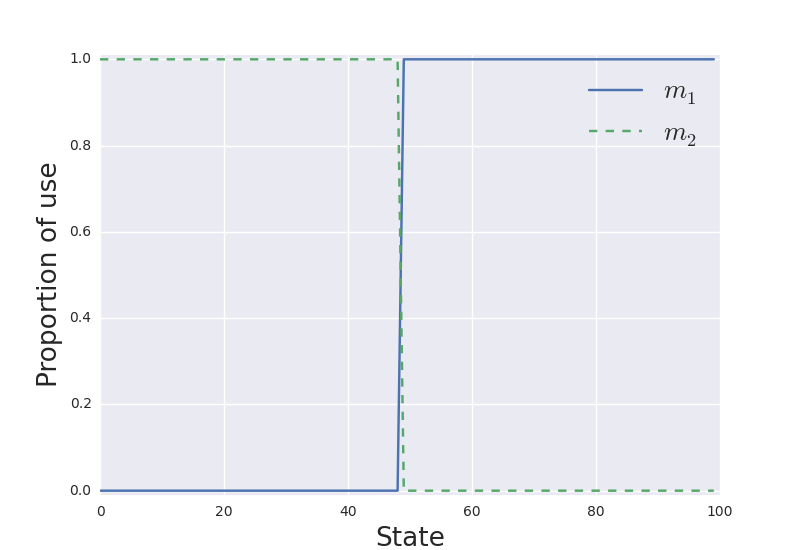
\includegraphics[scale=0.4]{../code/plots/vag-gen0.png}
    \caption{Initial non-vague population.}
    \label{fig:vaga}
  \end{subfigure}
  ~
   \begin{subfigure}[b]{0.45\textwidth}
    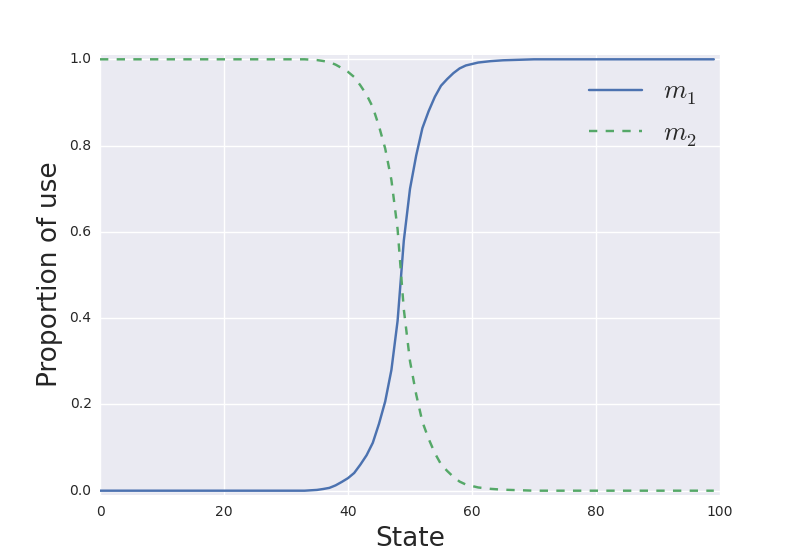
\includegraphics[scale=0.4]{../code/plots/vag-gen1.png}
    \caption{Vague population after single generation.}
    \label{fig:vagb}

  \end{subfigure}
  \caption{Noisy iterated learning with posterior sampling, $\sigma = 0.4$, and $k = 20$.}
  \label{fig:vag}
\end{figure}
 
\paragraph{Discussion.}
Transmission perturbations caused by the noisy perception of states reliably give rise to vagueness even if no borderline cases were initially part of a population's language. As modeled here, vagueness is not evidenced by particular types but at the population level. That is, it is not a property of individuals' languages, which make sharp distinctions inasmuch as perception allows it, but of aggregated linguistic behavior. Of course, the stabilization of a linguistic system or population on a particular vague/clear state partition may reasonably be expected to depend not only on the effects of learning, but also on the functional (dis)advantages that this partition brings about for its users. Functional pressure may therefore well be necessary for borderline cases to be kept in check. Which factor or combination thereof plays a more central role for the emergence of vagueness is an empirical question we do not address here. Instead, we see these results as adding strength to the argument that one way in which vagueness may arise is as a byproduct of interactions between agents that may occasionally err in their perception of the environment -- be it in interaction under functional pressure or in acquisition under a pressure for learnability. 

\subsection{Deflation}
Meaning deflation is a diachronic process by which a form's once restricted range of applicability broadens. Perhaps the most prominent example is Jespersen's cycle \citep{dahl:1979}, the process by which emphatic negation, such as French {\em ne ... pas}, broadens over time and instead becomes a marker for standard negation. As argued by \citet{bolinger:1981}, certain word classes are particularly prone to slight and unnoticed reinterpretation. Consequently, when retrieving their meaning from contextual cues, learners may continuously spread their meaning out. For instance, Bolinger discusses how the indefinite quantifier {\em several} has progressively shifted from meaning {\em a respectable number} to broader {\em a few} in American English. We follow this line of reasoning and show how state confusability may lead to meaning deflation.


\paragraph{Setup.} As above, $S = [0,99]$, each type is associated with an index $i \in [0,99]$,
and the noise pattern is given by $P(s_p|s_a) \sim \text{Normal}(s_{a},\sigma,s_{0},s_{99})$. However, we
now trace the change of a single message $m$, e.g., {\em several}, coupled with linguistic behavior such that
$P(m|s_j,t_i) = 1$ iff $j \geq i$. Otherwise no message is sent. This behavior
causes asymmetry in the learning data as types with high indices will reserve their message
only for a small subset of the state space and otherwise remain silent. Consequently, learning
also needs to be modified to take such silent observations into account. For simplicity, we
assume that learners are aware of $k$ and that
$P(t_i | d_l) \propto (\prod_{s \in d_l} P(m|s,t_i)) \times \text{Binom}(\text{successes} =
k-|d_l|, \text{trials} = k, \text{succ.prob} = \sum_{j=0}^{i-1} P(s_j))$.\footnote{Knowing fixed $k$ allows learners to compute the likelihood of a type not reporting $k -|d_l|$ state observations. A more involved but better justified alternative is to specify a prior over $k$ and for learners to perform a joint inference on $k$ and the teacher's type given a partial observation of only overtly produced data. For simplicity, we opt for the former, albeit admittedly artificial, assumption.}
As before, the former factor corresponds to the likelihood of a type producing the perceived 
data.  The latter is the probability of a type not reporting $k-|d|$ events for a
total of $k$ events. $P \in \Delta(S)$ is assumed to be uniform. In words, a long sequence of
data consisting of mostly silence gives stronger evidence for the type producing it having a
high index even if the few state-message pairs observed in the sequence may be equally
likely to be produced by types with lower indices.

\paragraph{Results.} The development of an initially monomorphic population consisting only of $t_{80}$ is shown in Figure \ref{fig:defl}. In this setup even little noise will cause a message to gradually be applied to larger portions of the state space. As above, the speed by which meaning deflates is regulated by $\sigma$, $k$, and to lesser degree $l$. In general, more state confusion due to higher $\sigma$, shorter sequences, or less posterior maximization will lead to more learners inferring lower types than present in the previous generation. 

\begin{figure}[ht]
\centering
    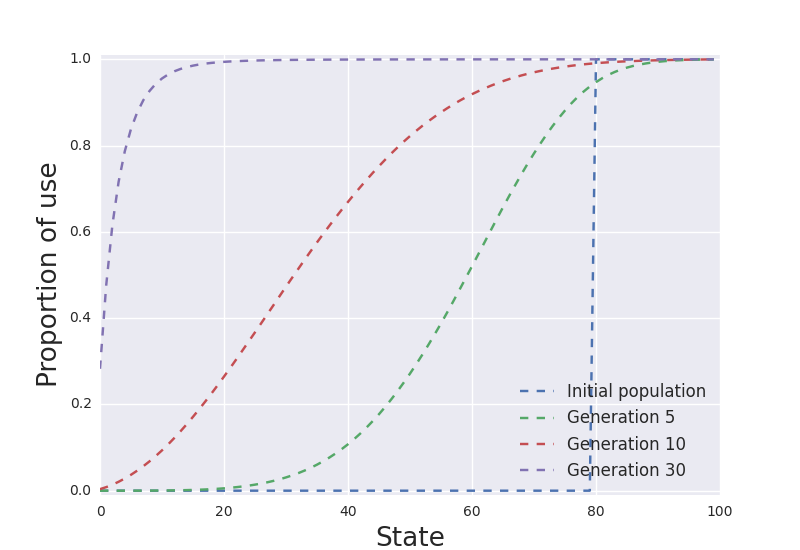
\includegraphics[scale=0.4]{../code/plots/deflation-sigma04.png}
  \caption{Noisy iterated learning with posterior sampling, $\sigma = 0.4$, and $k = 30$.}
  \label{fig:defl}
\end{figure}

\paragraph{Discussion.} In contrast to the previous case study, we now considered the effects of noisy perception under asymmetric data generation where overt linguistic evidence is not always produced. This setup can be likened to acquisition only from positive linguistic evidence in a world in which not every state is labeled. %(coupled with the idealized assumption that learners are aware of the amount of silence ``produced'' by a teacher). 

The overall result is similar to that of the previous study. Noisy perception can cause transmission perturbations that relax once strict linguistic conventions. In contrast to the case of vagueness, if there are no competing forms, e.g., {\em small} vs. {\em tall}, asymmetry in production and noise will iteratively increase the state space that a form carves out. Just as the overuse of a word or difficulties in the retrieval of its meaning from contextual cues may lead to the deflation of its meaning in natural language.


\subsection{Scalar expressions}
Scalar expressions have been at the center of many studies on pragmatic inference. Examples
include quantifiers such as {\em some} and {\em most}, adjectives such as {\em cold} and {\em
  big}, and numerals such as {\em four} and {\em ten}. Their commonality lies in that
their use is often taken to pragmatically convey an upper-bound that these expressions
semantically lack \citep{horn:1972,gazdar:1979}. For instance, while ``I ate some of the
  cookies'' is truth-conditionally compatible with a world state in which the speaker ate
all of them, this utterance is usually reasoned to convey that the speaker ate {\em some but
  not all}. Otherwise, she would have used {\em all}. In this way the
meaning of a scalar expression lacking an upper-bound is strengthened by interlocutors' mutual reasoning
about rational language use \citep{grice:1975}.

To explain the selection for a lack of upper-bounds in these expressions, \citet{brochhagen+etal:2016:CogSci} propose a model that combines functional pressure and iterated learning.  Crucially, this account requires the assumption of a prior that favors a lack of upper-bounds. Technically, this assumption is required to distinguish between a language that rules out the bound pragmatically, as English, and a hypothetical alternative that does so semantically. Let us call the former language $L_{\text{bound}}$ and the latter $L_{\text{lack}}$. To see the problem posed by $L_{\text{bound}}$ recall that learners need to infer unobservables from overt information. As a consequence, a user of $L_{\text{bound}}$ might be difficult to impossible to tease apart from one using $L_{\text{lack}}$ but conveying the bound pragmatically. In the following we focus on only these two languages to elucidate under which conditions noisy perception may lead to the selection of $L_{\text{lack}}$ without a cognitive bias nor functional pressure.


\paragraph{Setup.} We follow the setup of \citet{brochhagen+etal:2016:CogSci} with a reduced type space that only considers $L_{\text{bound}}$ and $L_{\text{lack}}$ paired with either literal or pragmatic language use. Both lexica specify the truth-conditions of two messages in either of two states. Let us mnemonically label them $\msome$, $\mall$, $\ssome$ and $\sall$, where the former state is one in which natural language {\em some but not all} holds, and the latter one where {\em all} holds. Consequently, in $L_{\text{bound}}$ message $\msome$ is only true of $\ssome$ and $\mall$ only of $\sall$. In English-like $L_{\text{lack}}$, message $\mall$ is also only true of $\sall$, but the meaning of $\msome$ is underspecified and lexically holds in both states. Following previous models of probabilistic rational language use lexica are paired with a linguistic behavior (c.f. \citealt{frank+goodman:2012, franke+jaeger:2014}). This behavior can either be literal or pragmatic, giving rise to the following choice probabilities of four different types (see \citealt{brochhagen+etal:2016:CogSci} for details):

\begin{centering}
\hspace{2.8cm} \underline{$L_{\text{bound}}$} \hspace{2.6cm} \underline{$L_{\text{lack}}$} \hspace{1cm}\\
Literal $\approx$ \hspace{0.6cm}  \bordermatrix{~ & \msome & \mall \cr 
                  \sall & 0 & 1 \cr
                  \ssome & 1 & 0 \cr} \hspace{0.5cm} \bordermatrix{~ & m_1 & m_2 \cr 
                  \sall & 0.5 & 0.5 \cr
                  \ssome & 1 & 0 \cr}\\[0.25cm]
Pragmatic $\approx$ \hspace{0.05cm}  \bordermatrix{~ & \msome & \mall \cr 
                  \sall & 0 & 1 \cr
                  \ssome & 1 & 0 \cr} \hspace{0.5cm} \bordermatrix{~ & m_1 & m_2 \cr 
                  \sall & 0 & 1 \cr
                  \ssome & 1 & 0 \cr},\\[0.5cm]
\end{centering}

where $P(m|s,t)$ corresponds to cell $M_{sm}$ of a type's choice matrix. These values, rounded here for better readability, are obtained by combining lexica with linguistic behavior and a rationality parameter $\lambda$. Intuitively, higher values of $\lambda$ increase the speaker's propensity to produce utterances that maximize communicative success. For our purposes this parameter is fixed to be reasonably high so as to render speaker behavior (mostly) deterministic ($\lambda = 20$). Pragmatic types are obtained through a process of mutual reasoning by which linguistic choice is refined, approximating the informal reasoning spelled out above. In this case a pragmatic $L_{\text{lack}}$ speaker pragmatically associates $\ssome$ more strongly with $\msome$ because she reasons (that her interlocutor reasons) that, if she wants to convey $\sall$ successfully, she would be better off using $\mall$. Lastly, and differently from Brochhagen et al.'s noise-free model, noise is introduced by parameters $\epsilon$ and $\delta$. The former corresponds to the probability of perceiving the actual state $\ssome$ as $\sall$, $P(\sall | \ssome) = \epsilon$, and $P(\ssome | \sall) = \delta$.

\paragraph{Results.} To quantify the effects of the dynamics we ran $50$ independent
simulations per parameter configuration. Each population was initialized with an arbitrary
distribution over types. The mean proportion of pragmatic users of $L_{\text{lack}}$ under
different noise signatures is shown in Figure \ref{fig:quant}. These results show that when
$\delta$ is small and $\epsilon$ is high, iterated noisy transmission can lead to populations
consisting of mostly, if not exclusively, a type that does not lexicalize an upper-bound for {\em some}-like expressions but conveys it pragmatically.  Similar results are obtained for
increments in $k$, $l$, or $\lambda$.

\begin{figure}[ht]
\centering
    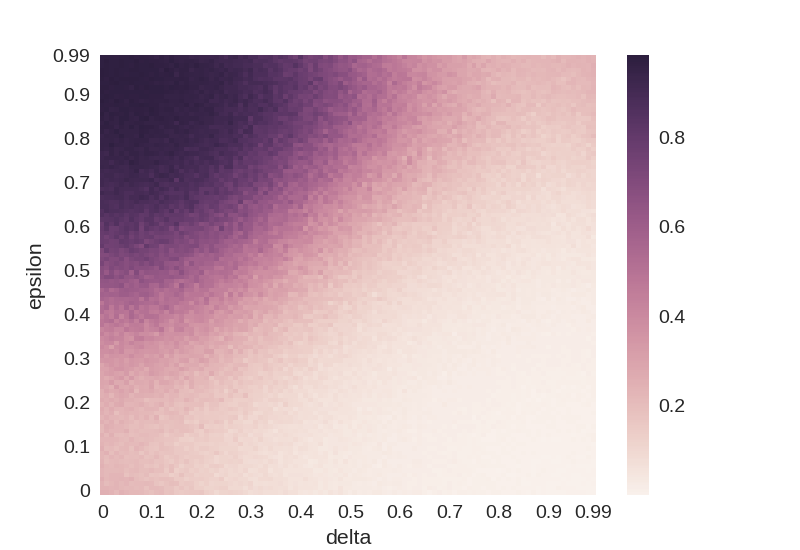
\includegraphics[scale=0.33]{../code/plots/quantifiers-posterior-sampling-k5.png}
  \caption{Mean proportion of pragmatic $L_{\text{lack}}$ users after $20$ generations with posterior sampling, $k = 5$, and $\lambda = 20$.}
  \label{fig:quant}
\end{figure}


\paragraph{Discussion.} The main goal of this case study was to show that noisy perception may mimic the effect of cognitive biases. In the case of Brochhagen et al. the assumed bias was one for simplicity. Accordingly, learners had an a priori preference for not codifying an upper-bound lexically. This increases the learners' propensity to infer pragmatic $L_{\text{lack}}$ over $L_{\text{bound}}$ even if the data witnessed could not tease them apart. Here, we assumed no such bias but nevertheless arrived at an evolutionary outcome that is comparable to the one predicted if the bias were present. Note however that this outcome strongly depends on the types involved. Whether a type thrives under a particular noise signature depends on the proportion of types confused with it during transmission. The addition or extraction of a single type may therefore lead to different results. 

At present, it is unclear what role noisy perception should play in the selection of underspecified meaning. These results should therefore be taken as suggestive but not indicative of a relationship between the two. A possible way to explore this relation may lie in their connection to empirical work on the verification of quantified statements (see \citealt{szymanik:2016} for a recent overview). The idea being that some states are easier to verify, e.g., $\sall$, and therefore less confusable with other states than others, e.g., $\ssome$. 


\section{General discussion}
We proposed a model of iterated Bayesian learning that accommodates for systematic noise in agents' perception, giving rise to stochastic perturbations that may influence and explain language change. We investigated the model's predictions in three case studies that show that iterated noisy transmission can lead to outcomes akin to those found in natural language. As stressed before, these results are not meant to suggest noisy perception to be the sole or main determinant of these phenomena. Instead, our aim was mainly conceptual and technical in nature. 

Beyond technical aspects, we foregrounded two intertwined issues in the cultural evolution of language. First, the fact that noise signatures may mimic the effects of cognitive biases has consequences for the interpretation of the outcomes of acquisition processes. Care must therefore be exercised in reading off the influence of possible cognitive learning biases from data obtained both in the wild and the laboratory. Second, and more importantly, these results may be seen as complementing and stressing the pivotal role of systematic transmission perturbations as explanatory and predictive devices of language change -- independent of the perturbation's source. They thereby strengthen and widen the scope of research on iterated learning by bringing attention to forces beyond inductive biases. 


\section{Conclusion}
Acquisition is a central force shaping linguistic structure. The consideration of the (imperfect) means by which such knowledge is transmitted is therefore crucial to our understanding of the cultural evolution of language. Here, we focused on one factor that may give rise to explanatory systematic stochastic perturbation in learning; agents' noisy perception of the world, and analyzed its effects in three case studies on (i) vagueness, (ii) meaning deflation, and (iii) underspecified lexical meaning. Our results suggest that the class of relevant perturbation sources reaches beyond the well-studied effects of inductive learning biases. In particular, that some linguistic properties, such as (i), (ii) and more tentatively (iii), may emerge as a byproduct of environmental factors that influence agents' perception of the world. 


\section{Acknowledgments}
\tb{TO DO}


\bibliographystyle{apacite}

\setlength{\bibleftmargin}{.125in}
\setlength{\bibindent}{-\bibleftmargin}

\bibliography{noise-bib}


\end{document}
